%\documentclass[tip_rada, jezik]{FSBtex}
% moguce opcije su:
%	-> tip_rada: seminar, zavrsni, projekt, diplomski
%	-> jezik (dodatni parametar, moze i bez njega ako se pise na hrvatskom): hrvatski, engleski
\documentclass[zavrsni]{FSBtex}


\usepackage{lipsum}

% naredbe za generiranje datoteke
% pdflatex main.tex
% bibtex main
% makeindex -s nomencl.ist -o main.nls main.nlo
% makeglossaries-lite main
% pdflatex main.tex
% pdflatex main.tex


% postavke rada
\author{Marko Markić}

\mentor{prof. dr. sc. Miki Mikić, dip. ing.}
\mentorDva{dr. sc. Pero perić, dip. ing.}

\zahvala{
Izjavljujem da sam ovaj rad izradio samostalno koristeći stečena znanja tijekom studija i navedenu literaturu.\\

Zahvaljujem se svom mentoru \textbf{prof. dr. sc. Peri Periću} što mi je omogućio da napišem ovaj rad......
}


\zadatak{slike/zadatak.pdf}

\kljucnerijeci{PID; LQR; hidraulika}
\keywords{PID; LQR; hydraulics}

%----------------------------------------------------------------------------------------
%	POCETAK DOKUMENTA
%----------------------------------------------------------------------------------------
\begin{document}
\NaslovnaStrana	% ova naredba ukljucuje sve naslovne strane rada ovisno o tipu rada, te sadrzaj i popise slika i tablica

% u slucaju enegleske verzije potrebno obrnut redoslijed sazetaka
\begin{sazetak}
Ovdje ide sažetak rada na hrvatskom\\
\end{sazetak}

\begin{abstract}
Ovdje ide sažetak rada na engleskom jeziku\\
\end{abstract}


% sve sa A se prvo ispisuje kod oznaka
\nomenclature[A]{$s$}{klizna površina SMC regulatora \nomunit{\si{\kilogram\per\cubic\meter}}}
\nomenclature[A]{$k_1,\ k_2$}{pojačanja SMC regulatora \nomunit{-}}%
\nomenclature[A]{$k_1,\ k_2,\ k_3$}{pojačanja metode povratnog koraka \nomunit{-}}%

% konstante
\nomenclature[C]{$g$}{gravitacijsko ubrzanje  \nomunit{9,81 \si{\meter\per\square\second}}}%

%% grcke oznake
\nomenclature[G]{$\beta,\ \gamma$}{težinski koeficijenti PID regulatora \nomunit{-}}%
\nomenclature[G]{$\rho$}{gustoća fluida, \nomunit{\si{\kilogram\per\cubic\meter}} }%

% indeksi
\nomenclature[I]{$\alpha_d$}{koeficijent istjecanja \nomunit{-}}%

% akcenti
\nomenclature[T]{$\underline{\square}$}{Dual quaternion }%

% kratice
\newacronym{ga}{GA}{genetski algoritmi (eng. \textit{Genetic Algorithms})}
 
 

 
 
%----------------------------------------------------------------------------------------
%	OVDJE IDE OSTATAK RADA I SVA POGLAVLJA
%----------------------------------------------------------------------------------------
% pocetak brojanja rada od prve stranice
\pagebreak
\setcounter{page}{1}
\pagenumbering{arabic}

% ovdje ide ostatak rada
\chapter{Uvod}
Jedan od najznačajnijih problema kod konstruiranja mehanizama je optimalna sinteza mehanizma.
Tijekom godina razvijeno je nekoliko metoda za sintezu mehanizama \cite{Chiang2000, Hansen2009} ali svaka od njih primjenjiva je samo na određenim tipovima mehanizma. 
Zbog toga odabir odgovarajuće metode optimiranja mehanizma ovisi o samom mehanizmu koji se želi optimirati tj. aplikaciji mehanizma, potrebnoj numeričkoj točnosti te vremenu koje je potrebno da se postigne optimalno riješenje.

Primjena mehanizma utječe na optimizacijski problem, tj. ograničuje ga. U industrijskim aplikacijama ta ograničenja su dužine elemenata, prostor u koji mehanizam mora stati...\\

Možemo razlikovati dvije vrsta optimalne sinteze mehanizma: dimenzionalna i strukturalna sinteza. 
Dimenzionalna sinteza svodi se na određivanje dimenzija linkova mehanizma koji će omogućiti slijeđenje željene trajektorije ili funkcije, dok su mehanizam i veze između linkova poznati.
Strukturalna sinteza teži je problem jer nam nije poznat mehanizam ni veze između linkova te stoga moramo optimirati i topologiju i dimenzije mehanizma.\\

U ovom radu koristiti će se \acrlong{ga} ili \acrshort{ga} \cite{McCall2005, Cabrera2002} za optimiranje mehanizma.
Referenca na primjer tablice~\ref{tbl:primjer}.


\begin{table}[h!]
\centering
\caption{Primjer tablice}
\label{tbl:primjer}
\begin{tabular}{ccc}
stupac 1 & stupac 2 & stupac 3\\
\hline
\hline
nesto & $a+b$ & nesto\\
$a+b$ & nesto & $a+b$\\
\hline
\end{tabular}
\end{table}
\chapter{Izvod matematičkog modela}

Za mehanizam sa slike \ref{fig:mehanizma} potrebno je izvršiti optimalnu sintezu dimenzija mehanizma tako da bi moment na ručici $A_0A$ bio konstantan. U cilindru se nalazi idealni plin i cijeli proces se odvija pri konstantnoj temperaturi. Zadane su slijedeće vrijednosti:
\begin{align*}
h_1&=250\ \text{mm}\\
h_2&=75\ \text{mm}\\
F_1&=18\ \text{N}\\
\Delta \varphi &=\frac{\pi}{3}\\
A&=konst
\end{align*}

\begin{figure}[H]
\center
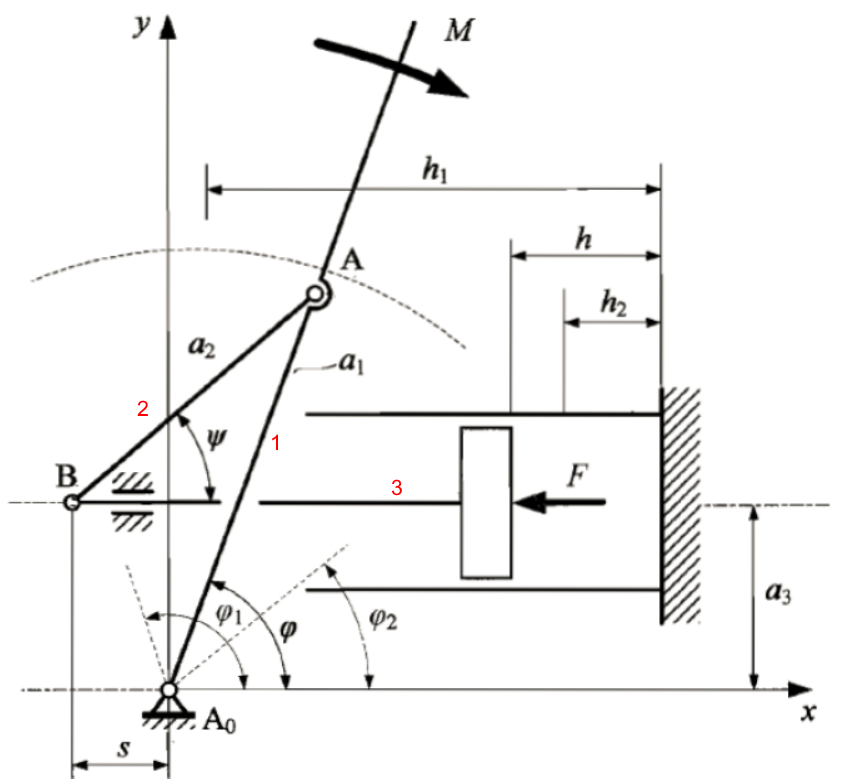
\includegraphics[scale=.4]{slike/mehanizam.png}
\caption{Skica mehanizma za optimiranje}
\label{fig:mehanizma}
\end{figure}

\section{Izvod funkcije cilja}
\quad Za konstantu temperaturu i eksponent politrope $n=1$ dobivamo ravnotežnu promjenu stanja kod koje se temperatura radnog medija ne mijenja tj. $T_1=T_2=T$ i $\Delta T=0$.\\

Jednadžbe stanja:
\begin{equation}
\label{eq:stanje1}
p_1V_1=mRT_1
\end{equation}
\begin{center}
i
\end{center}
\begin{equation}
\label{eq:stanje2}
p_2V_2=mRT_2
\end{equation}

povezane uvjetom $T_1=T_2=T$ daju sljedeću jednadžbu stanja:
\begin{equation}
\label{eq:stanje}
p_1V_1=p_2V_2=pV
\end{equation}

Volumen u cilindru računa se prema formuli \ref{eq:volumen} dok se sila na klip računa po izrazu \ref{eq:sila}.
\begin{equation}
\label{eq:volumen}
V=Ah
\end{equation}
\begin{equation}
\label{eq:sila}
F=pA
\end{equation}

Uvrstimo li izraze \ref{eq:volumen} i \ref{eq:sila} u jednadžbu \ref{eq:stanje} dobije se slijedeća jednadžba:
\begin{gather}
\dfrac{F_1}{A}h_1A=\dfrac{F_2}{A}h_2A=\dfrac{F}{A}hA\\
\label{eq:sile_polozaj}
F_1h_1=F_2h_2=Fh
\end{gather}

Iz zadanih vrijednosti i izraza \ref{eq:sile_polozaj} možemo izračunati silu $F_2$ (\ref{eq:F2}) te općeniti izraz za silu u ovisnosti o položaju klipa (\ref{eq:F}).
\begin{gather}
F_2=F_1\dfrac{h_1}{h_2}=18\dfrac{250}{75}\\
\label{eq:F2}
F_2=60\ N\\
\nonumber \\
F=F_1\dfrac{h_1}{h}=18\dfrac{250}{h}\\
\label{eq:F}
F=\dfrac{4500}{h}\ \text{N/mm}
\end{gather}

Nakon što smo dobili općeniti izraz za silu u ovisnosti o položaju možemo izraziti moment o ovisnosti o sili i položaju klipa preko elementarnih radova:
\begin{equation}
Md\varphi + Fdh=0
\end{equation}
\begin{equation}
M=-F\dfrac{dh}{d\varphi }=-\dfrac{4500}{h}\dfrac{dh}{d\varphi}
\end{equation}


Redukcijom sile na prvi član mehanizma (slika \ref{fig:mehanizma}) dobije se reducirani moment
\begin{equation}
\label{eq:reducirani}
M_{red}=F\dfrac{dh}{d\varphi }=\dfrac{4500}{h}\dfrac{dh}{d\varphi }
\end{equation}
tj. treba biti $M+M_{red}=0$.\\

Zbog toga traži se minimalno odstupanje funkcije $M(\varphi)=\dfrac{4500}{h}\dfrac{dh}{d\varphi }$ pri gibanju od $\varphi_1$ do $\varphi_2$.
Pomoću zadanog područja gibanja $\delta\varphi$ možemo izračunati konstantni moment:
\begin{gather}
d\varphi=\dfrac{4500}{M(\varphi )}\dfrac{dh}{h}\\
\nonumber\\
\varphi_1 - \varphi_2=\dfrac{4500}{M(\varphi)}ln\left(\dfrac{h_1}{h_2}\right)\\
\nonumber\\
M_{konst}=\dfrac{3\cdot 4500}{\pi}ln\left(\dfrac{250}{75}\right)=5173,69\ \text{Nmm}
\end{gather}

U ovom slučaju nam je zadatak minimizirati funkciju cilja $f(\varphi)=M(\varphi)-M_{konst}$.


\section{Kinematika mehanizma}

\quad Kinematička shema mehanizma s ishodištem koordinatnog sustava u točki $A_0$ prikazana je na slici \ref{fig:mehanizma}. Kod kinematičke analize mehanizma važno je unaprijed definirati koordinatni sustav i u skladu s njim paziti na predznake pomaka, sila idt. \\
Na osnovi kinematičkog modela sastavlja se matematički model za računanje kinematičkih veličina potrebnih za optimizaciju. To su položaj klipa $s$ odnosno $h$, kut $\varphi$ i derivacija $ds/dh=dh/d\varphi$.\\

Računanje položaja klipa $s$ pomoću prijenosnih funkcija mehanizma:
\begin{gather}
a_1sin(\varphi)+a_2sin(180+\psi)-a_3=0\\
\nonumber \\
sin(\psi) = \dfrac{a_1}{a_2}sin(\varphi)-\dfrac{a_3}{a_2}\\
\nonumber \\
sin(\psi) = k_1sin(\varphi)-k_2\\
\end{gather}
gdje su:
\begin{itemize}
\item $a_1=\sqrt{A_x^2+A_y^2}$
\item $a_2=\sqrt{(A_x-B_x)^2+(A_y-B_y)^2} $
\item $\varphi=atan\left( \dfrac{A_y}{A_x}\right) $
\item $k_1=\dfrac{a_1}{a_2}$
\item $k_2=\dfrac{a_3}{a_2}$
\end{itemize}

\begin{gather}
a_1cos(\varphi)+a_2cos(180^\circ+\psi)+scos(0)=0\\
\nonumber \\
s = a_2cos(\psi)-a_1cos(\varphi)\\
\nonumber \\
\label{eq:s}
s = -a_1cos(\varphi)+a_2\sqrt{1-(k_1sin(\varphi)-k2)^2}
\end{gather}

Iz jednadžbe \ref{eq:s} moramo izračunati derivaciju $ds/d\varphi$:
\begin{equation}
\label{eq:dsdfi}
\dfrac{ds}{d\varphi}=a_1sin(\varphi) - \dfrac{a_2k_1cos(\varphi)\left( k_1sin(\varphi)-k_2\right) ^2}{\sqrt{1-(k_1sin(\varphi)-k_2)^2}}
\end{equation}







\chapter{Optimiranje mehanizma}
Nakon što smo dobili matematički model kinematike mehanizma moramo odrediti projektne varijable. U ovom slučaju će projektne varijable biti koordinate točaka $A$ i $B$ mehanizma:
$x_1=A_x$, $x_2=A_y$, $x_3=B_x$ i $x_4=B_y=a_3$.\\

Nakon što smo odredili projektne varijable moramo odabrati slučajni početni položaj mehanizma za koji ćemo izračunati dužine linkova mehanizma, početni kut mehanizma te za odabrano područje gibanja i odabrani broj koraka u području gibanja računa se vrijednost funkcije cilja uz zadana ograničenja mehanizma.\\

Ograničenja mehanizma za ovaj zadatak su slijedeća:
\begin{align*}
g_1&=x_1-25\geq 0\  &g_2=45-x_1\geq 0\\
g_3&=x_3+15\geq 0\   &g_4=5-x_3\geq 0\\
g_5&=x_2-5\geq 0\  &g_6=25-x_2\geq 0\\
g_7&=x_4-5\geq 0\   &g_8=25-x_4\geq 0\\
\end{align*}

U ovom radu usporediti će se dvije funkcije cilja:
\begin{enumerate}
\item $f(\varphi)=max\left( \mid M_{konst}-M(\varphi)\mid\right) $
\item $f(\varphi)=\sum_{i=1}^{n}\left( M_{konst}-M_i(\varphi) \right)$
\end{enumerate}

Da bi mehanizam mogli optimirati pomoću genetskog algoritma moramo problem minimizacije svesti za na problem maksimizacije te tada optimizacijski problem za genetski algoritam glasi:
\begin{equation}
max \rightarrow \dfrac{1}{1+f(\varphi)}
\end{equation}
\chapter{Rezultati}


\section{Minimizacija najvećeg odstupanja}
\quad Za genetski algoritma sa slijedećim parametrima: 
\begin{itemize}
\item vjerojatnost križanja $0,7$
\item vjerojatnost mutacije $0,02$
\item veličina populacije $100$
\item broj iteracija $50000$
\item funkcija cilja $f(\varphi)=max\left( \mid M_{konst}-M(\varphi)\mid\right) $
\end{itemize}
dobiveni su slijedeći rezultati:
\begin{itemize}
\item početne koordinate točke $A(383,46\quad 70,47)$ i točke $B(-138,45\quad  92,32)$ u mm
\item maksimalni moment od $5191,7$ Nmm te minimalni moment od $5155,7$  Nmm
\item vrijednost funkcije cilja $0,0526$
\end{itemize}

Prikaz dijagrama momenta može se vidjeti na slici \ref{fig:max_m1},a funkcije cilja na slici \ref{fig:max_f1}. Najveća apsolutna razlika u odstupanju od željene vrijednosti momenta iznosi približno $18$ Nmm što je vrlo zadovoljavajuće za ovaj mehanizam.


\begin{figure}[h!]
\center
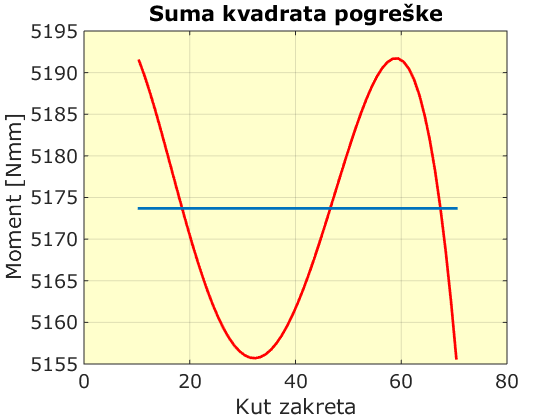
\includegraphics[scale=.6]{slike/max_m1.png}
\caption{Dijagrama odstupanja momenta od traženog (prvi set parametra)}
\label{fig:max_m1}
\end{figure}

\begin{figure}[h!]
\center
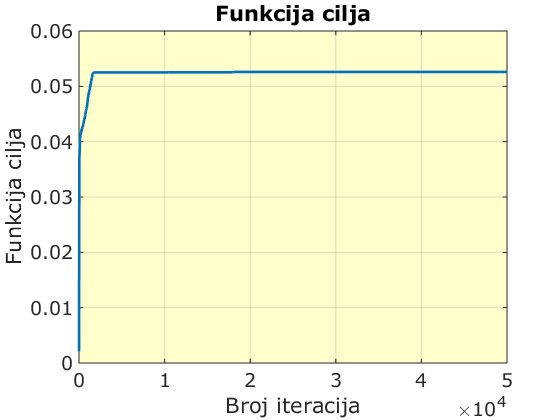
\includegraphics[scale=.6]{slike/max_f1.png}
\caption{Prikaz funkcije cilja (prvi set parametra)}
\label{fig:max_f1}
\end{figure}




\quad Drugi set parametara algoritma dan je sa slijedećim parametrima: 
\begin{itemize}
\item vjerojatnost križanja $0,7$
\item vjerojatnost mutacije $0,01$
\item veličina populacije $100$
\item broj iteracija $10000$
\item funkcija cilja $f(\varphi)=max\left( \mid M_{konst}-M(\varphi)\mid\right) $
\end{itemize}
te su dobiveni su slijedeći rezultati:
\begin{itemize}
\item početne koordinate točke $A(380,28\quad 72,63)$ i točke $B(-137,51\quad  91,57)$ u mm
\item maksimalni moment od $5192,5$  Nmm te minimalni moment od $5154,8$  Nmm
\item vrijednost funkcije cilja $0,0606$
\end{itemize}


Prikaz rezultata za drugi set parametara može se vidjeti na slikama \ref{fig:max_m2} i \ref{fig:max_f2}. Najveća apsolutna razlika u odstupanju od željene vrijednosti momenta iznosi približno $18,8$ Nmm što je vrlo zadovoljavajuće za ovaj mehanizam.

\begin{figure}[h!]
\center
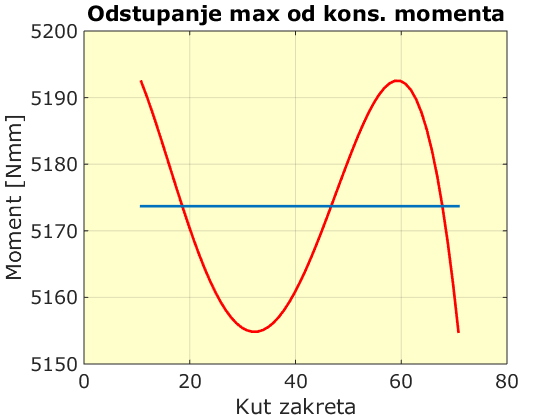
\includegraphics[scale=.6]{slike/max_m2.png}
\caption{Dijagrama odstupanja momenta od traženog (drugi set parametra)}
\label{fig:max_m2}
\end{figure}

\begin{figure}[h!]
\center
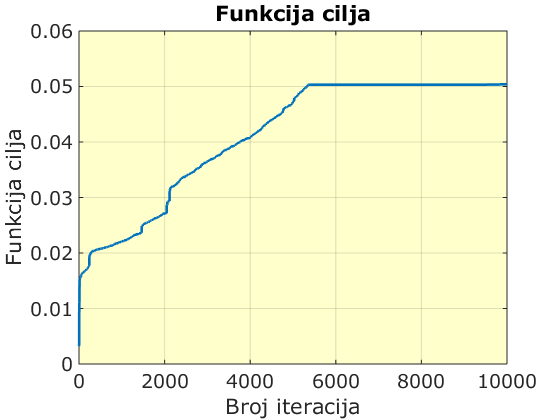
\includegraphics[scale=.6]{slike/max_f2.png}
\caption{Prikaz funkcije cilja (drugi set parametra)}
\label{fig:max_f2}
\end{figure}



\section{Suma kvadrata pogreške}

\quad Treći set parametara algoritma dan je sa slijedećim parametrima: 
\begin{itemize}
\item vjerojatnost križanja $0,7$
\item vjerojatnost mutacije $0,02$
\item veličina populacije $100$
\item broj iteracija $50000$
\item funkcija cilja $f(\varphi)=\sum_{i=1}^{n}\left( M_{konst}-M_i(\varphi) \right)$
\end{itemize}
te su dobiveni su slijedeći rezultati:
\begin{itemize}
\item početne koordinate točke $A(409,21\quad 50)$ i točke $B(-148,88\quad  99,26)$ u mm
\item maksimalni moment od $5182,9$  Nmm te minimalni moment od $5152,3$  Nmm
\item najveća apsolutna razlika u odstupanju od željene vrijednosti iznosi $21,39$ Nmm
\end{itemize}


\begin{figure}[h!]
\center
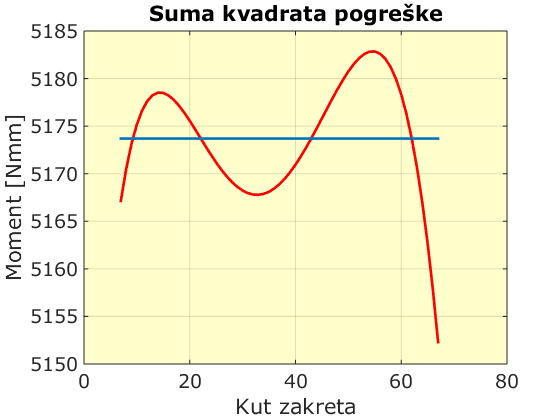
\includegraphics[scale=.6]{slike/sum_m1.png}
\caption{Dijagrama odstupanja momenta od traženog (treći set parametra)}
\label{fig:sum_m1}
\end{figure}

\begin{figure}[h!]
\center
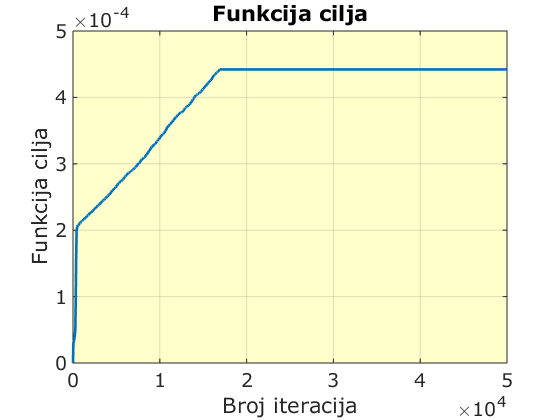
\includegraphics[scale=.6]{slike/sum_f1.png}
\caption{Prikaz funkcije cilja (treći set parametra)}
\label{fig:sum_f1}
\end{figure}



\quad Četvrti set parametara algoritma dan je sa slijedećim parametrima: 
\begin{itemize}
\item vjerojatnost križanja $0,7$
\item vjerojatnost mutacije $0,01$
\item veličina populacije $100$
\item broj iteracija $50000$
\item funkcija cilja $f(\varphi)=\sum_{i=1}^{n}\left( M_{konst}-M_i(\varphi) \right)$
\end{itemize}
te su dobiveni su slijedeći rezultati:
\begin{itemize}
\item početne koordinate točke $A(409,21\quad 50)$ i točke $B(-148,88\quad  99,26)$ u mm
\item maksimalni moment od $5182,9$ Nmm te minimalni moment od $5152,3$  Nmm
\item najveća apsolutna razlika u odstupanju od željene vrijednosti iznosi $21,38$ Nmm
\end{itemize}


\begin{figure}[h!]
\center
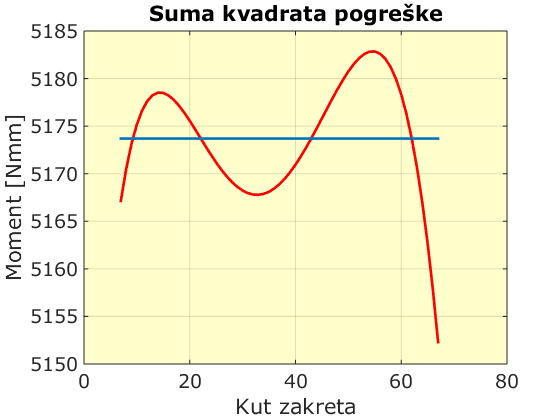
\includegraphics[scale=.6]{slike/sum_m2.png}
\caption{Dijagrama odstupanja momenta od traženog (četvrti set parametra)}
\label{fig:sum_m2}
\end{figure}

\begin{figure}[h!]
\center
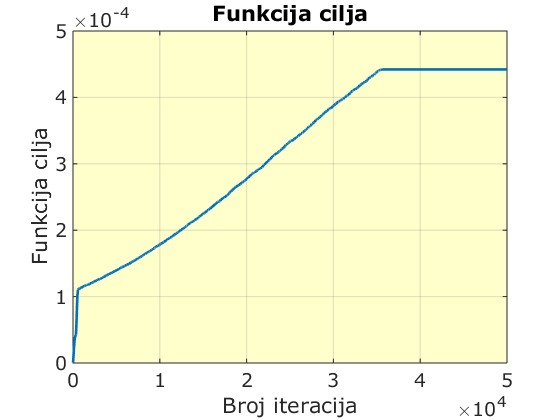
\includegraphics[scale=.6]{slike/sum_f2.png}
\caption{Prikaz funkcije cilja (četvrti set parametra)}
\label{fig:sum_f2}
\end{figure}


Sa slika \ref{fig:sum_m1} i \ref{fig:sum_m2} možemo vidjeti da momentni dijagrama za sumu kvadrata izgledaju isto i imaju iste vrijednosti. Isto tako možemo vidjeti da za vjerojatnost križanja od $0,01$ algoritmu treba puno više iteracija za konvergenciju ka točnom rješenju.



\chapter{Zaključak}
Ovdje ide zaključak rada





% literatura:
\LiteraturaPostavke
\bibliography{literatura}


\appendix
\chapter{Matematički izvodi}
Ovdje ide prilog koji isto moze imati svoju tex datoteku!
Ukoliko je u radu potrebno definirati teorem on se može definirati na slijedeći način:
\begin{theorem}[Proba]
Ovdje ide neki tekst
\begin{equation}
c^2 = a^2+b^2ˇ
\end{equation}
\end{theorem}

Isto vrijedi i za definiciju
\begin{definition}[adf]
Umetni neki tekst
\begin{equation}
c^2 = a^2+b^2ˇ
\end{equation}
\end{definition}



\end{document}





